\scanpage{18}
\begin{flushright}\handwritten{\unsure{1.9.3|1.93|1.9.5}, \unsure{1.27|1.23}, 2.9 to be transferred to \unsure{numbe\textsuperscript{r} 3}\unsure{?}\\3.1}\end{flushright}

\(\mathbb{S}\)GA 4 VI

\uline{Contents}
\margin{\handwritten{\uline{\unsure{pp|pv|pr}}}}

1. Finiteness conditions for the objects and arrows of a topos.\margin{\handwritten{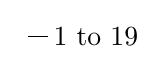
\begin{tikzpicture}[baseline=0,x=.45cm,y=.45cm]\draw (-.7,.12)--(-.15,.12);\node[anchor=west,inner sep=0pt] at (0,.12) {1 to 19};\end{tikzpicture}}}

2. Finiteness conditions for a topos.\margin{\handwritten{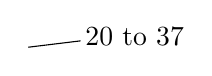
\begin{tikzpicture}[baseline=0,x=.45cm,y=.45cm]\draw (-1.6,-.18)--(-.12,0);\node[anchor=west,inner sep=0pt] at (0,.12) {20 to 37};\end{tikzpicture}}}

3. Finiteness conditions for a morphism of topoi. \deleted{\handwritten{Case of \unsure{inductive|induced} \unsure{topoi}}}\margin{\handwritten{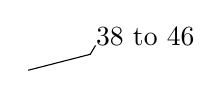
\begin{tikzpicture}[baseline=0,x=.45cm,y=.45cm]\draw (-1.9,-.5)--(-.15,-.05)--(0,.2);\node[anchor=west,inner sep=0pt] at (0,.45) {38 to 46};\end{tikzpicture}}}

\deleted{4. Constructibility.}\inserted{\handwritten{4. Finiteness conditions for a topos \inserted{obtained by} gluing.}}\margin{\handwritten{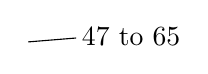
\begin{tikzpicture}[baseline=0,x=.45cm,y=.45cm]\draw (-1.5,-.03)--(-.15,.08);\node[anchor=west,inner sep=0pt] at (0,.12) {47 to 65};\end{tikzpicture}}}
% The pencil divider is immediately beneath the original and replacement item 4.
\noindent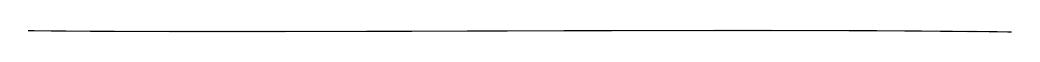
\begin{tikzpicture}[x=\linewidth,y=.4cm]\draw (-.07,0)..controls (.2,-.08) and (.7,.08)..(.96,-.04);\end{tikzpicture}
% The relocation curve remains in the LEFT margin, with its question mark;
% its lower end is beside the circled replacement 5 and its arrowhead points
% to the divider after item 4. The drawing preserves the source's relative geometry.
\reversemarginpar
\margin{\handwritten{\begin{tikzpicture}[x=.55cm,y=.55cm]
\draw[->] (2,-6.5)..controls (-1,-4.6) and (-1,-3.2)..(2,0);
\node at (.05,-1.8) {?};
\end{tikzpicture}}}
\normalmarginpar

\deleted{5}\handwritten{6}. Fibered categories and $\underset{\handwritten{\longrightarrow}}{\mathrm{Lim}}$ (reminders).

\deleted{6}\handwritten{7}. Fibered sites and topoi.

\reversemarginpar
\margin{\handwritten{
\begin{tikzpicture}[x=.45cm,y=.45cm]
\draw (1,0)..controls (1,-.8) and (1,-1.0)..(.62,-1.03)
 ..controls (1.2,-1.25) and (.9,-2.1)..(1.16,-2.32);
\end{tikzpicture}}}
\normalmarginpar
\deleted{7}\handwritten{8}. Projective limits of topoi.

\deleted{8}\handwritten{\unsure{8|9}}. Case of filtering projective limits of coherent topoi with coherent transition morphisms: theorems on passage to the limit for cohomology.

\noindent\begin{tikzpicture}[baseline=(n.base)]\node[draw,ellipse,inner sep=3pt] (n) {\deleted{9}\handwritten{5}.};\end{tikzpicture} Cohomology of an inductive limit of shea\unsure{\deleted{x}v|\deleted{v}x}es on a coherent topos
% The right edge cuts immediately after the t of cohérent; no full stop is visible.

\reversemarginpar
\margin{\handwritten{\begin{tikzpicture}[x=.25cm,y=.25cm]\draw[line width=2pt] (0,0)--(.04,-.55);\end{tikzpicture}}}
\normalmarginpar
\handwritten{10. Appendix (by P. Deligne). \deleted{Existence of point\unsure{s}} \unsure{\deleted{of }A|\deleted{of A}} coherent topos \unsure{has} \inserted{enough points}\unsure{.}}

\deleted{NB \(\mathbb{B}\)eyond doubt \deleted{\unsure{9|8}}\handwritten{8} would be interchangeable with the block \deleted{5}\handwritten{4} to \deleted{8}\handwritten{9}. But it seems more natural to me to put in two consecuti\unsure{\deleted{s}v|\deleted{v}s}e numbers the two facets o\unsure{\deleted{y}f|\deleted{g}f|\deleted{f}y|\deleted{f}g} the \unsure{\deleted{b}p|\deleted{p}b|\deleted{l}p|\deleted{p}l}assage to the limit in cohomology. Of cou\unsure{\deleted{t}r|\deleted{r}t}se, number \deleted{\unsure{9}}\handwritten{8} will be reduced to one or two pages, the sorites of finiteness conditions having already been done.}

\deleted{Numbe\textsuperscript{\uline{r}} 4 will contain the sorites of constructible groups (in the sense of groups finite or not), of torsion sheaves, of notions of constructibility for Modules and complexes of Modules, - including the special facts in the locally noetherian case. I think I shall write it up but do not guarantee it. One can \deleted{at a pinc} dr\deleted{\unsure{l|i}}\handwritten{o}p numbe\textsuperscript{\uline{r}} 4, it will then be less beautiful of course ...:}

\deleted{The following write-up of numbe\textsuperscript{\uline{r}}s 1 to 3 is ào\unsure{\deleted{p}m|\deleted{m}p}plete, except that I intend to add a few more examples to it (in particular a locally algebraic non-algebraic topos\inserted{\handwritten{)}}\unsure{,|.} \deleted{a non-coherent morphism of coherent topoi).}}
\reversemarginpar
\margin{\handwritten{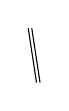
\begin{tikzpicture}[x=.3cm,y=.3cm]\draw (0,0)--(.35,-2.3);\draw (.15,0)--(.5,-2.3);\end{tikzpicture}}}
\normalmarginpar
\unsure{\inserted{\handwritten{and a topos having a generating family consisting of coherent object\unsure{s}, which is not locally algebraic}}}
% The outer unsure on the bottom insertion records live/cancelled-state uncertainty.
% archive sheet number: 17
